% !TeX root = ../main.tex
\section{Introduction}

For a long time, China has left behind a large number of historical documents, which have very important academic and artistic value. 
Therefore, in recent years, the study of historical documents has received widespread attention from researchers~\cite{jinic21,hde,obc306}. 

Different from other text recognition tasks, historical document recognition tasks face unique challenges like complexity and damage to the characters in historical documents, including stains, tears, and ink bleeding. 
In addition to the complexity of text recognition of historical documents, another major problem comes from the data itself. Specifically, history document recognition suffers from the long-tailed character occurrence distribution~\cite{obc306mk2}. 
The long-tailed distribution also affects other text recognition tasks like~\cite{fudanvi}, however, historical document recognition suffers a larger ``longtailness'' measured by the Gini Coefficient~\cite{tailsurvey}(See Figure~\ref{fig:moretailed}). 
Furthermore, novel characters can appear in the testing data~\cite{jinic21}, making it a hybrid of zero-shot and long-tail problems.

\begin{figure}[!t]
	\centering
	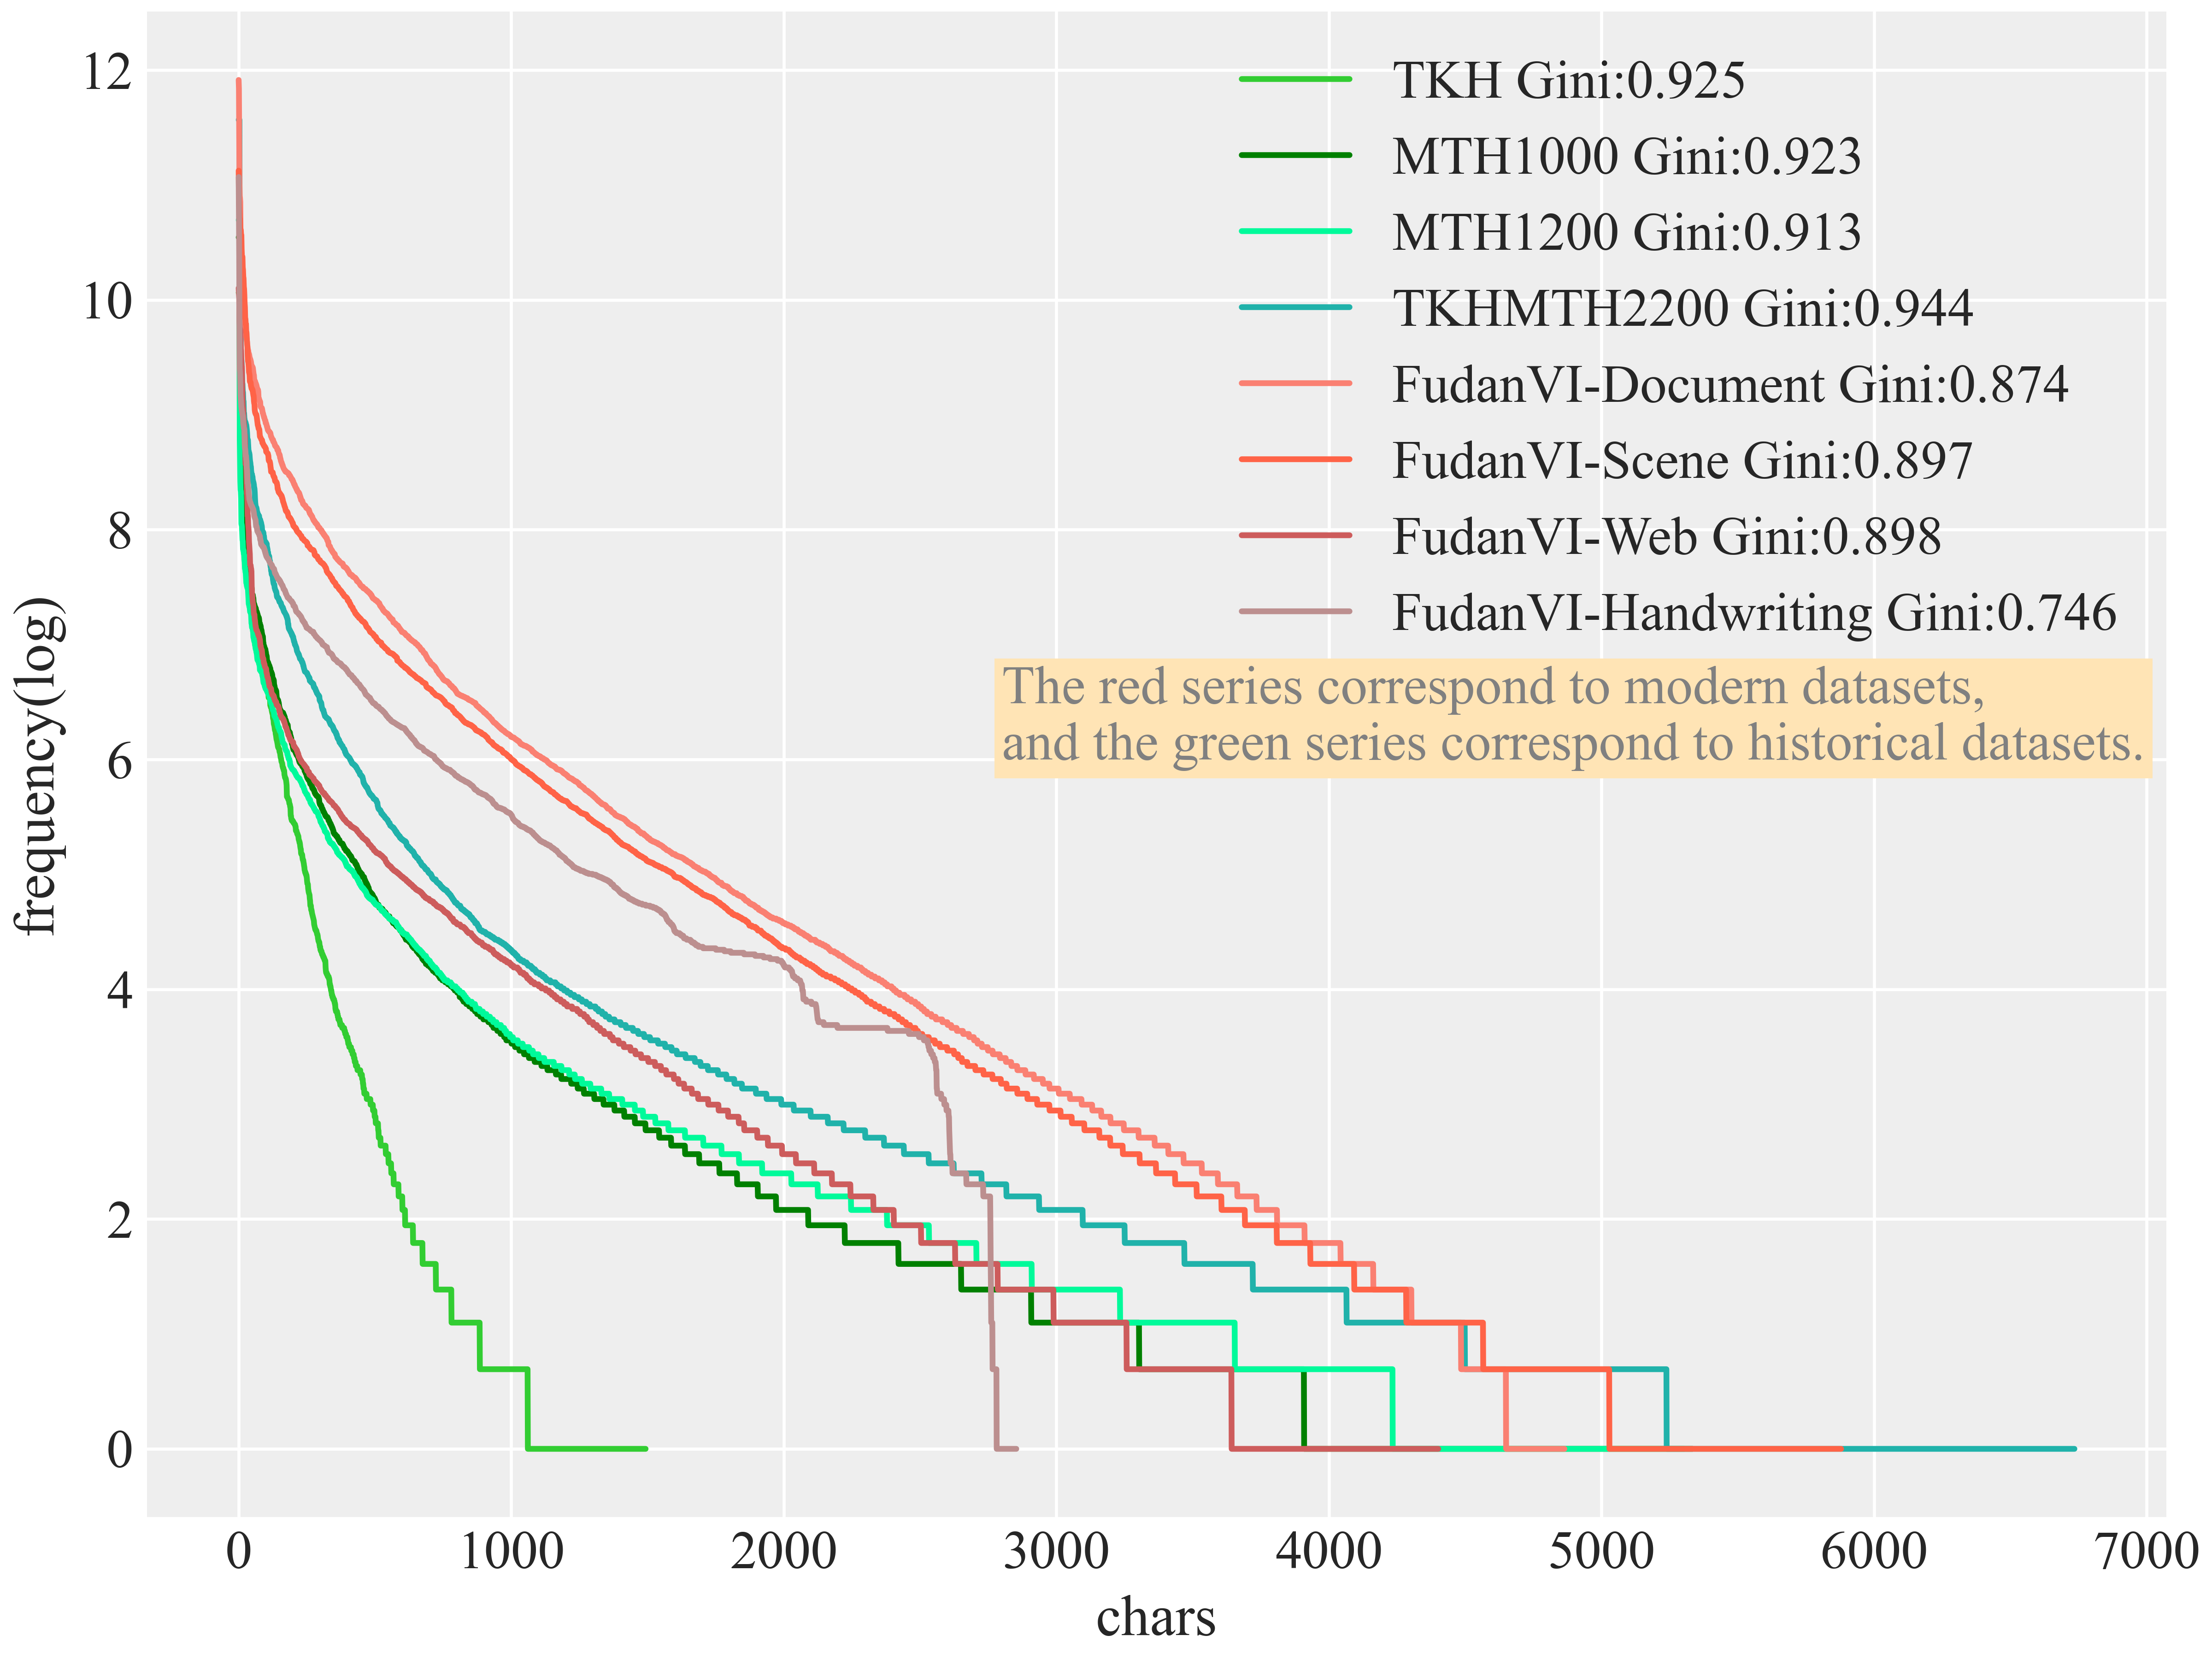
\includegraphics[width=\linewidth]{figures/database_long_tail.png}
	\caption
    {Comparison on Gini Coefficient~\cite{tailsurvey} between modern text recognition datasets~\cite{fudanvi} and historical text recognition datasets~\cite{tkhmth}.}
	\label{fig:moretailed}
\end{figure}

To address this challenge, existing methods propose to exploit the radical information of each character~\cite{denseran}, where individual radicals are often used in both head and tail (including unseen) classes, which are shown to generalize well in recognizing the novel characters~\cite{fewran,zhang20pr}.
On the other hand, Zhang et. al.~\cite{sanicdar23}  proved that exploiting the component information can improve the performance of tail classes.
However, such methods depend on radical-level annotations to train, yielding expensive annotation costs to deploy.

In this work, we propose to break free from the radical annotation by adopting a visual matching approach~\cite{vsdf}. 
To keep exploiting the similarity of character components, we propose implicitly emphasizing detail feature modeling.  
Specifically, we propose the spindle backbone network, which increases the number of parameters to layers corresponding to component features~\cite{mobile}. 
We argue character parts are more similar to texture patterns, which are more modeled in middle layers (conv2 and conv3) according to~\cite{dissection}.
On the other hand, high-frequency signals are reported harmful to the generalization~\cite{hfharm,hffilter}, hence we refrain from making shallow layers wider. 
The network also reduces the parameters in deeper layers to keep the total parameter to keep a small vram footprint and high inference speed.

Summarizing the above motivations, we propose a spindle network that has narrower shallow and deep layers but a wider middle layer. 

The results indicate that the design effectively improves the model performance on tail classes, and also head classes.  
We also conducted architectural ablative experiments, which verified that the spindle design is better than the usual pyramid design and the reverse pyramid design in terms of performance, justifying our motivation.

As a structural-knowledge-free approach, the proposed method also possesses decent recognition capability on novel classes, which can reduce the efforts needed for adapting the model for new excavations. In addition, the approach also helps improve the head classes as well. 

In summary, the main contributions of this paper can be considered as follows:
\begin{enumerate}[noitemsep]
    \item We found that the similarity of character components can be leveraged to improve the performance of tails in long-tail distribution data.
    \item We implement a spindle network to extract character component features, exploiting the similarity between character components to improve the performance of tail classes.
    \item We conduct extensive experiments on three challenging Chinese ancient book datasets (TKH, MTH1000, and MTH1200) to validate the superiority of our proposed method. The results show that our approach achieves state-of-the-art performance in this field.
\end{enumerate}

\begin{figure*}[t]
    \begin{center}
    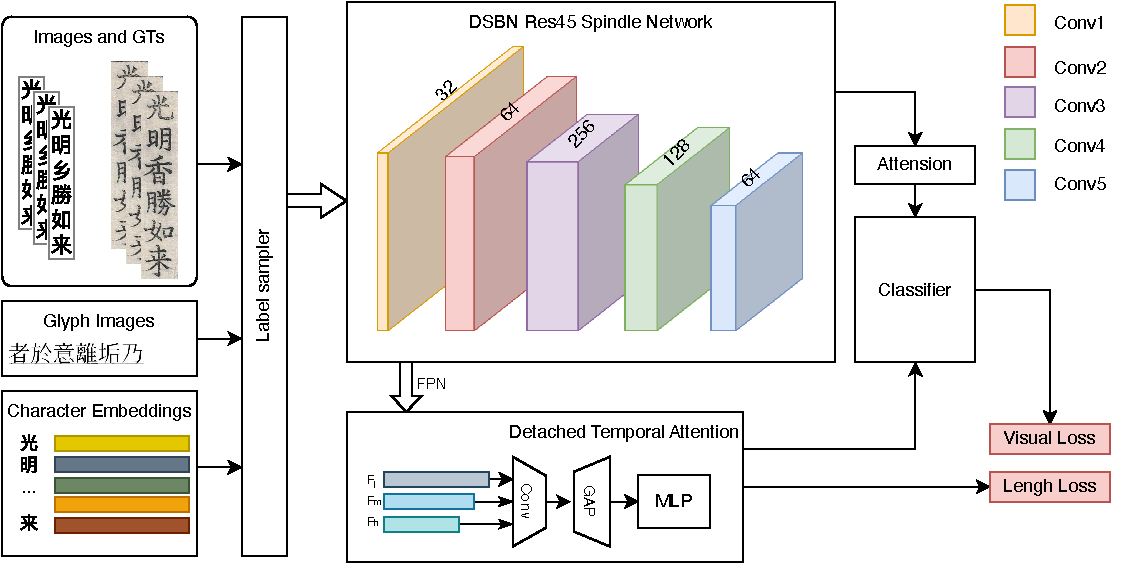
\includegraphics[width=1.0\linewidth]{figures/overall.pdf}
    \end{center}
    \caption{just a placeholder}
    \label{fig:overall}
\end{figure*}

    